\newpage
\section{Introduction}
When computing a result over a data type, a small change would lead to completely recomputing the result. Parts of the recomputation results in the same results as the previous computation. By keeping track of the intermediate results and then reusing the result when part of the data type is the same, would lead to less computation. 

An example of computing a result over a data type is computing the \textbf{binary tree maximum path sum}. Given a \texttt{Tree}, starting at the root node, find a path from top to bottom that leads to the maximum total.
\begin{haskell}
data Tree = Leaf Int
          | Node Tree Int Tree 
\end{haskell}

\begin{haskell}
exampleTree :: Tree    
exampleTree = Node (Node (Leaf 8) 7 (Leaf 9)) 3 (Node (Leaf 5) 4 (Leaf 2))
\end{haskell}

\begin{figure}[H]
    \centering
    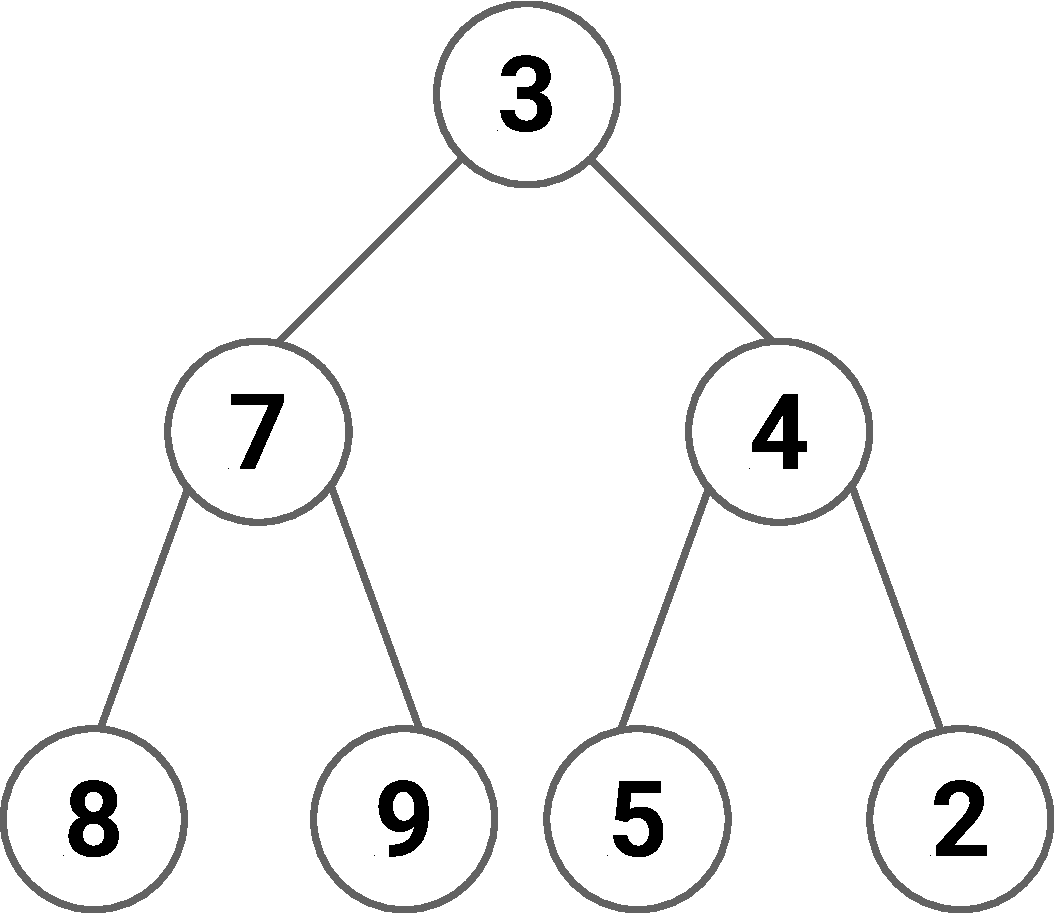
\includegraphics[width=.4\textwidth]{Tree.pdf}
    \caption{Graphic visualization of the \inlinehaskell{exampleTree}}
\end{figure}

An implementation of computing the max path sum over data type \texttt{Tree} is:

\todo[inline]{This function does not work for negative values}
\begin{haskell}
maxPathSum :: Tree -> Int
maxPathSum (Leaf x)     = x
maxPathSum (Node l x r) = x + max (maxPathSum l, maxPathSum r)
\end{haskell}

\newpage
And computing the max path sum over the \inlinehaskell{exampleTree} results in 19.

\begin{figure}[H]
\begin{minipage}[c]{0.35\textwidth}
\begin{haskell}
maxPathSum exampleTree !$\equiv$! 19
\end{haskell}
\end{minipage}
\hspace{0.1\textwidth}
\begin{minipage}[c]{0.55\textwidth}
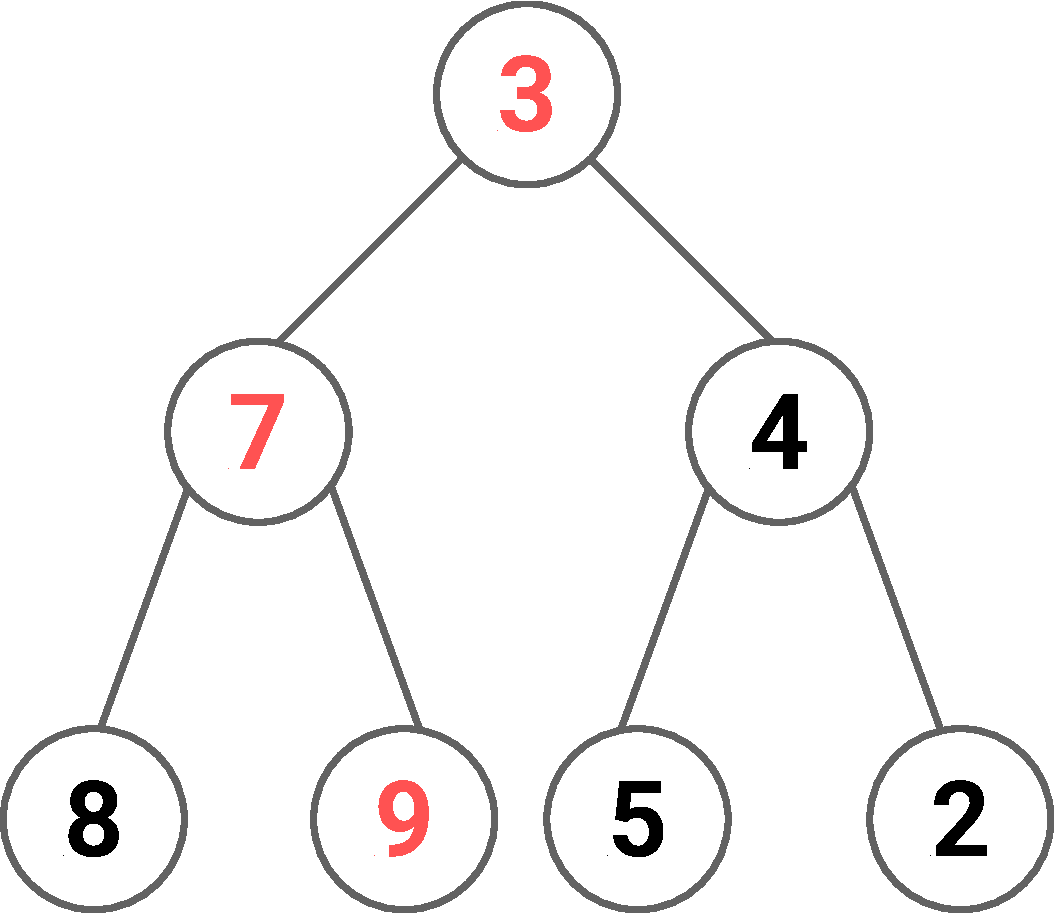
\includegraphics[width=0.7\textwidth]{SolvedTree.pdf}
\end{minipage}
\end{figure}

\todo[inline]{Add function complexities to the explanation}
To store the intermediate results of the computation of the max path sum, first, the \texttt{Tree} needs to be decorated for every \inlinehaskell{Node} and \inlinehaskell{Leaf} with a hash of its underlying structure. An implementation of decorating a \texttt{Tree} is:

\begin{haskell}
data MerkleTree = LeafH Hash Int
                | NodeH Hash Tree Int Tree

merkle :: Tree -> MerkleTree
merkle (Leaf x)     = LeafH (hash ["Leaf", x]) x
merkle (Node l x r) = NodeH (hash ["Node", x, hl, hr]) l' x r'
  where
    hl = getHash l'
    hr = getHash r'
    l' = merkle l
    r' = merkle r
\end{haskell}

\begin{figure}[H]
    \centering
    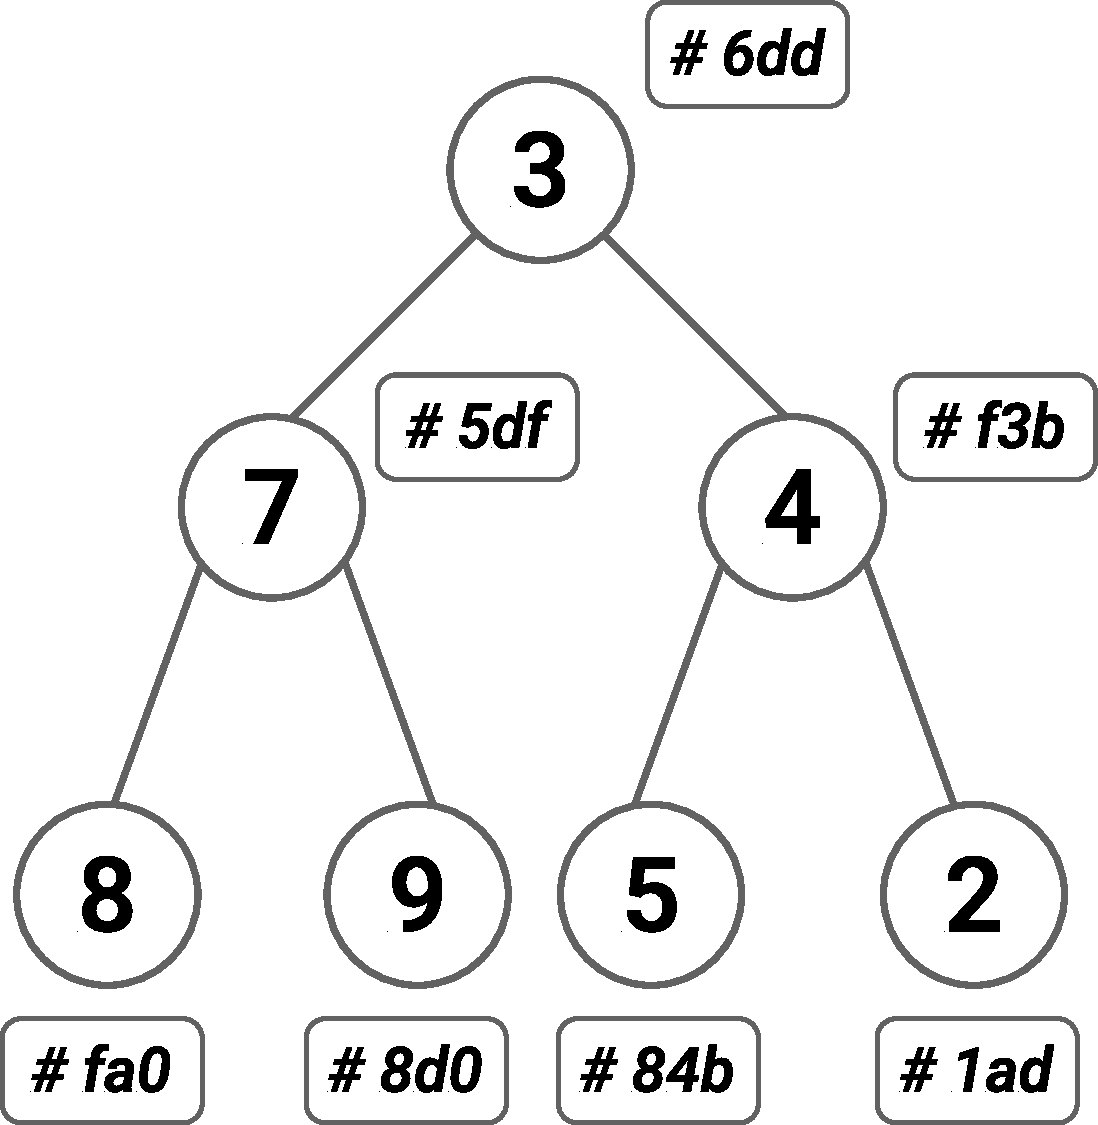
\includegraphics[width=.32\textwidth]{MerkleTree.pdf}
    \caption{The \texttt{MerkleTree} of \inlinehaskell{exampleTree}}
\end{figure}

Then using the precomputed hashes of the \texttt{MerkleTree}, a \texttt{Map} of intermediate results can easily be created by:

\begin{haskell}
maxPathSumInc :: MerkleTree -> (Int, Map Hash Int)    
maxPathSumInc (LeafH h x)     = (x, insert h x empty)
maxPathSumInc (NodeH h l x r) = (y, insert h y (ml <> mr))  
  where
    y = x + max (xl, xr)
    (xl, ml) = maxPathSumInc l
    (xr, mr) = maxPathSumInc r
\end{haskell}
\vspace{15pt}
\begin{figure}[H]
    \begin{minipage}[c]{0.55\textwidth}
        \centering
        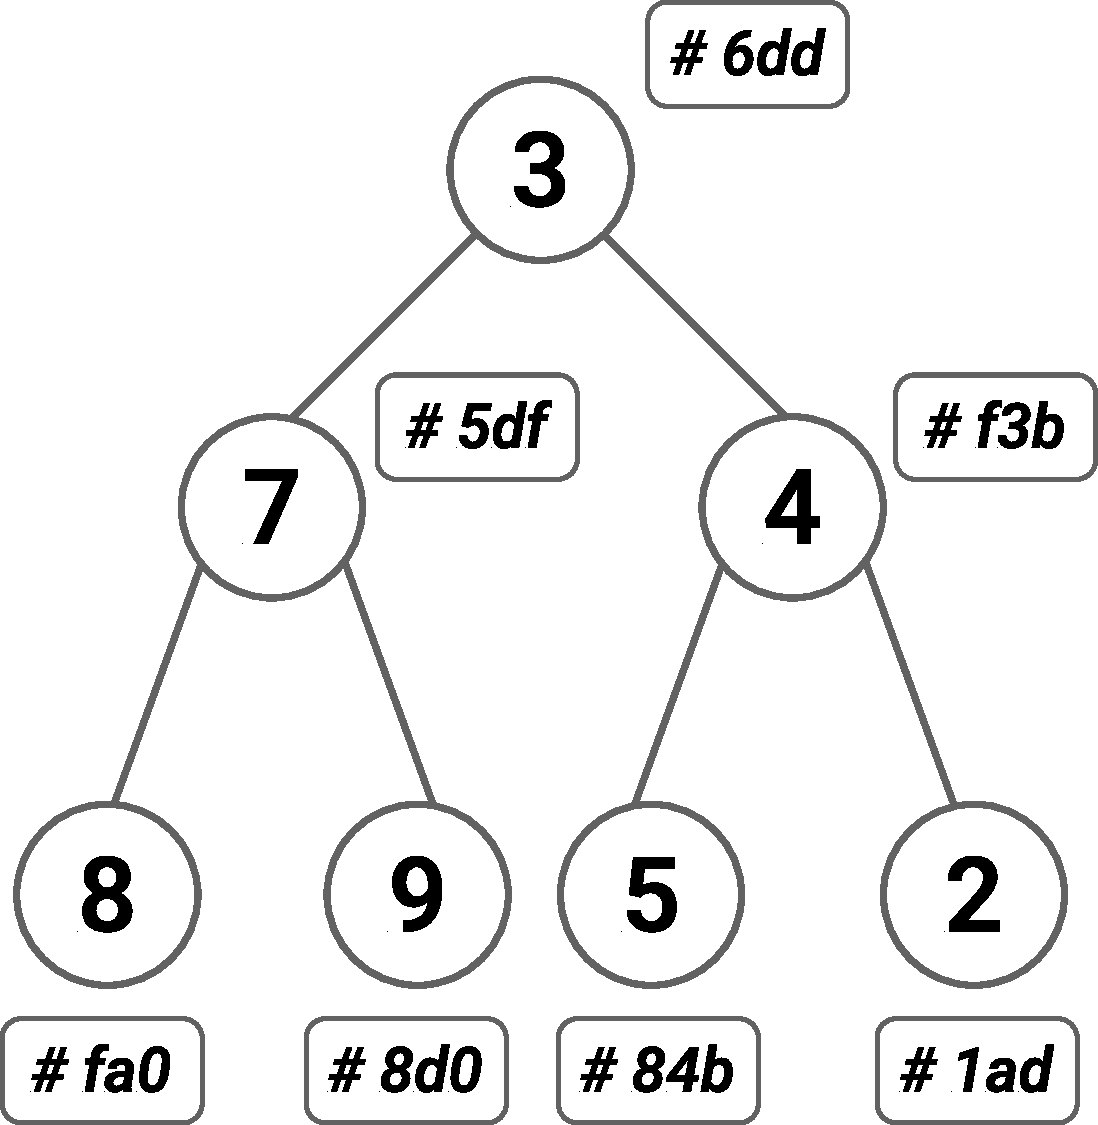
\includegraphics[width=.7\textwidth]{MerkleTree.pdf}
    \end{minipage}
    \hspace{0.1\textwidth}
    \begin{minipage}[c]{0.35\textwidth}
        \centering
        \begin{tabular}{|l|r|}
            \hline
            \textbf{Hash Nodes} & \textbf{Max Sum} \\
            \hline
            \# 6dd & 19 \\
            \hline
            \# 5df & 16 \\
            \hline
            \# fa0 & 8 \\
            \hline
            \# 8d0 & 9 \\
            \hline
            \# f3b & 9 \\
            \hline
            \# 84b & 5 \\
            \hline
            \# 1ad & 2 \\
            \hline
        \end{tabular}
    \end{minipage}
    \caption{The \texttt{MerkleTree} with intermediate results}    
\end{figure}

When there is a change in the \texttt{Tree}, only a part of the node hashes needs to be rehashed.

\begin{figure}[H]
    \centering
    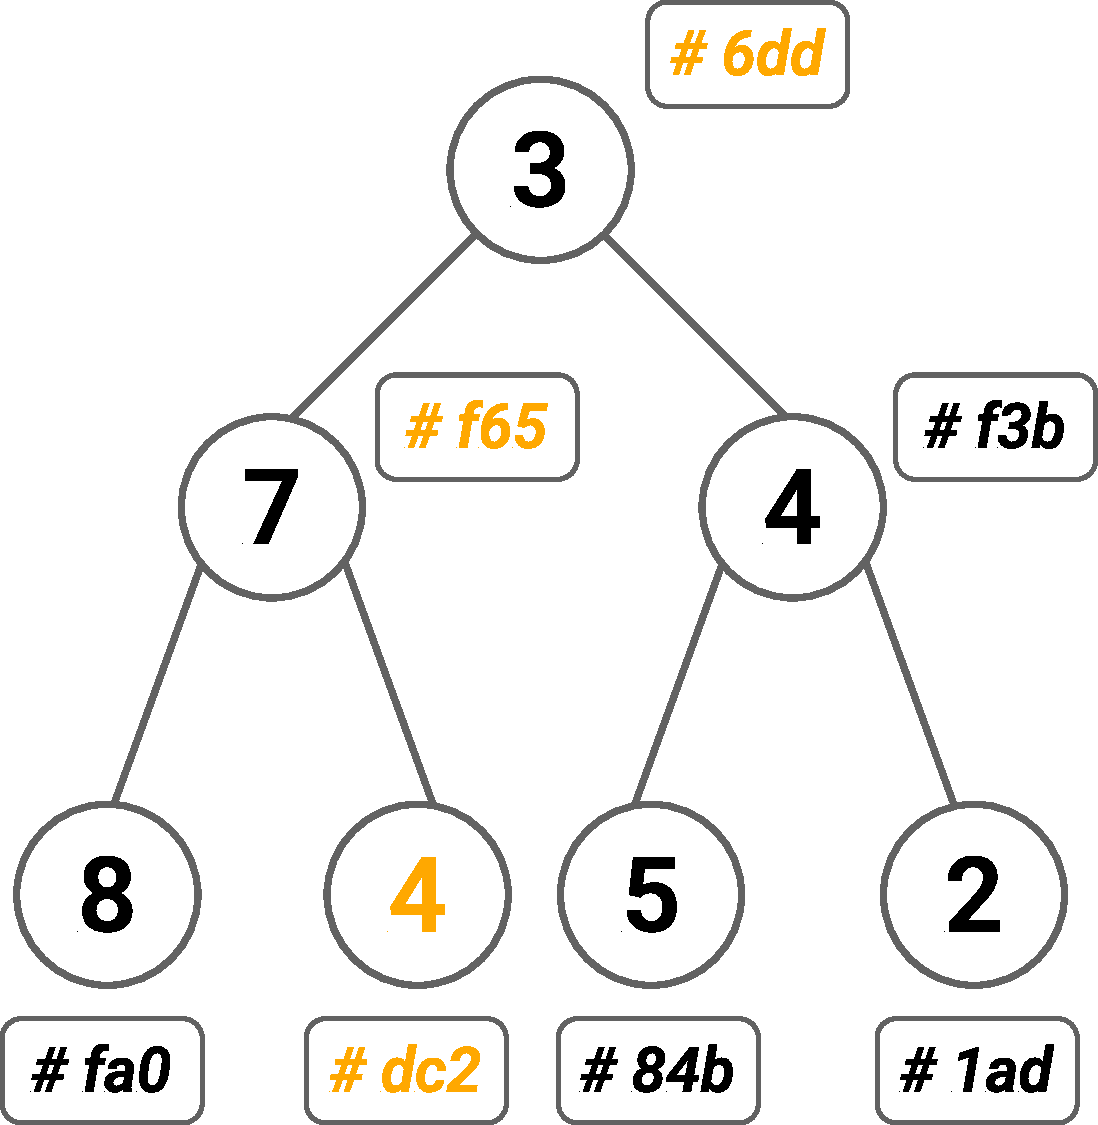
\includegraphics[width=.33\textwidth]{ChangedMerkleTree.pdf}
    \caption{Changed Tree}
\end{figure}

Then to compute the max path sum over the Changed Tree, the previously computed \texttt{Map} can be used to reduce the amount of recomputation.  

\begin{haskell}
maxPathSumMap :: Map Hash Int -> MerkleTree -> (Int, Map Hash Int)
maxPathSumMap m (LeafH h x) = case lookup m h of
  Just y  -> (y, m)
  Nothing -> (x, insert h x m)
maxPathSumMap m (NodeH h l x r) = case lookup m h of
  Just y  -> (y, m)
  Nothing -> (y, insert h y (ml <> mr))
    where
      y = x + max (xl, xr)
      (xl, ml) = maxPathSumMap m l
      (xr, mr) = maxPathSumMap m r  
\end{haskell}

In this paper, an implementation of storing the intermediate results is presented, supporting generic data types. That means the developer only needs to implement the max path sum functionality and the intermediate results are automatically stored.

\subsection{Contributions}
\begin{enumerate}[label={(\Alph*)}]
    \item A library needs to be implemented which contains the generic \texttt{merkle}, \texttt{cataMerkle} and \texttt{cataMerkleWithMap} functions
\end{enumerate}

\subsection{Research Questions}
Using the previously mentioned library, there is a multitude of questions to be answered:
\begin{enumerate}[label={(\Alph*)}]
    \item What parameters can be tweaked to have the best ratio of performance and memory usage?
    \item What type of equivalence is needed to reuse the incremental computation?
    \item What type of data structures are the best for storing the incremental computation?
    \item Could the library be used to perform static analysis in a more performant manner?
\end{enumerate}